   \begin{frame}{\ft{Oxy}}

        \begin{annotatedFigure}{0pt}{0pt}
            {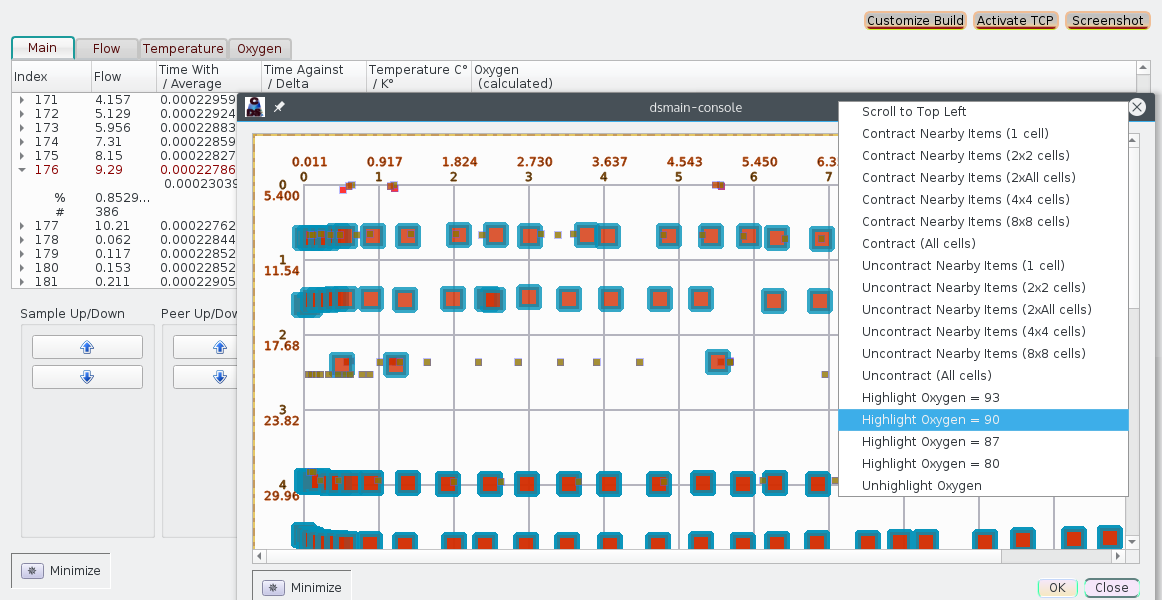
\includegraphics[scale=1]{texs/oxy.png}}
            
  \node [text width=7.6cm,align=justify,fill=logoCyan!20, draw=logoBlue, 
  draw opacity=0.5,line width=1mm, fill opacity=0.9]
   at (0.74,0.465){\textbf{Dataset Applications make extensive 
   use of context menus to organize functionality and provide 
   advanced interactivity.  In this screenshot a context menu 
   action (\circled{1}) has been selected which alters the 2D 
   display, visually emphasizing a restricted set 
   of data points (\circled{2}) and contracting all others (\circled{3}).}};

            \annotatedFigureBox{0.73,0.26}{0.96,0.328}{1}{0.89,0.326}%            
            \annotatedFigureBox{0.55,0.4}{0.55,0.44}{3}{0.55,0.44}            
            \annotatedFigureBox{0.598,0.45}{0.598,0.48}{2}{0.598,0.45}    
      %      \annotatedFigureBox{0.222,0.284}{0.3743,0.4934}{B}{0.3743,0.4934}%tr
      %      \annotatedFigureBox{0.555,0.784}{0.6815,0.874}{C}{0.555,0.784}%bl
      %      \annotatedFigureBox{0.557,0.322}{0.8985,0.5269}{D}{0.8985,0.5269}%tr
  
        \end{annotatedFigure}

   %     \caption{Expanded Sample (A)}
    %    \label{fig:teaser}

    \end{frame}

